\begin{center}\large\textbf{Readings: 9.1-9.5 326-360}\\
\normalsize \end{center}
\large \hlinewd{2pt}
~\\\textit{\textcolor{blue}{For the next section or two we will consider experiments that have quantitative responses and categorical predictors only (i.e. experiments that can be analyzed using ANOVA).  To start with let`s just look at a completely randomized experimental design (i.e. when analysis using one-way ANOVA could be done).  We will look at contrasts of the parameters that will lead directly into the way to analyze multi-way ANOVA models.}}\\~\\

Consider the traditional balanced One-Way ANOVA model.  That is, we have a \textit{continuous} response, $Y$, and a \textit{qualitative or categorical} predictor which we call our \textbf{factor}.  This factor has $t$ \textit{levels} (also the \textit{treatments} in this case) and our interest lies in whether or not the mean response differs between the treatments.\\~\\
The parametrization of the One-way ANOVA model we have looked at is
$$Y_{ij}=\mu+\tau_{i}+E_{ij},~~i=1,2,...t,~~j=1,...,n_{i},$$
$E_{ij}\sim N(0,\sigma^2)$ (balanced implies $n_{i}$ is the same for all levels).  The (true) treatment mean for treatment $i$ is given by $\mu+\tau_{i}=\mu_{i}$.\\~\\
Consider the bovine antibiotic/binding percentage example from earlier.  Let 
\begin{eqnarray*}
\mu_{1}& = & \mu+\tau_{1} =  \mbox{mean of Chloramphenicol treatment}\\
\mu_{2}& = & \mu+\tau_{2} =  \mbox{mean of Erythromycin treatment}\\
\mu_{3}& = & \mu+\tau_{3} =  \mbox{mean of Penicillin G treatment}\\
\mu_{4}& = & \mu+\tau_{4} =  \mbox{mean of Streptomycin treatment}\\
\mu_{5}& = & \mu+\tau_{5} =  \mbox{mean of Tetracyclin treatment}
\end{eqnarray*}

There were four observations at each treatment level.  Recall the p-value for testing the global hypothesis that 
$$H_0: \tau_1=\tau_2=\tau_3=\tau_4=\tau_5=0~~~~vs~~~~H_A:\mbox{At least 1 differs}$$
which is equivalent to testing 
$$H_0: \mu_1=\mu_2=\mu_3=\mu_4=\mu_5=0~~~~vs~~~~H_A:\mbox{At least 1 differs}$$
was $<0.0001$ implying we should reject $H_0$ in favor of $H_A$.  That is, at the 5\% significance level there is enough evidence to conclude the mean for at least one of the antibiotics differs.\\~\\
Given the answer to the previous question, the next logical question to answer is: `Which treatment means are different?'  Suppose we want first inspect the difference between the Cholramphenicol ($\mu_{1}$) and Erythromycin treatment means ($\mu_{2}$).  In terms of $\mu_{1}$ and $\mu_{2}$, how can we write this question as a null and alternative hypotheses?\\
\color{red}{$$H_{0}: \mu_1-\mu_2=0~~~\mbox{or}~~~\mu_1=\mu_2~~vs~~H_{A}:\mu_1-\mu_2\neq 0~~~\mbox{or}~~~\mu_1\neq\mu_2$$}
\color{black}{
This is an example of a \textbf{linear combination} of treatment means.  In general, a linear combination of treatment means takes the form}
\color{red}{
    $$\theta=c_{1}\mu_{1}+c_{2}\mu_{2}+...+c_{t}\mu_{t}$$
where the $c_{i}$ are called the coefficients of the linear combination (similar to linear combinations of the $\beta$'s we looked at in MLR and GLM).}\\~\\
\color{black}
For the bovine experiment, which of the following are linear combinations of treatment means?
\begin{itemize}
    \item $\theta_6=4\mu_{1}+3\mu_{2}-7\mu_{5}$ %yes
    \item $\theta_7=3\mu_{1}\mu_{4}+2\mu_{3}$     %no
    \item $\theta_8=\mu_{1}+\mu_{2}+\mu_{3}+\mu_{4}+\mu_{5}$  %yes
    \item $\theta_9=\mu_{1}^2+3\mu_{2}+1$   %no
\end{itemize}
If the coefficients of the linear combination sum to zero (i.e. $c_1+c_2+...+c_t=0$), the linear combination is called a \textbf{contrast}.\\~\\
Is our linear combination $\mu_1-\mu_2=0$ a contrast?  How about any of $\theta_6$ through $\theta_9$?\\\\~\\~\\~\\~\\~\\
If we want to do inference about a linear combination of treatment means we need an estimator of $\theta$, call it $\hat{\theta}$ and we will also need a measure of variability, say $\hat{SE}(\hat{\theta})$.\\~\\
An estimator is given by substitution of the sample means: 
    $$\hat{\theta}=c_{1}\bar{Y}_{1+}+c_{2}\bar{Y}_{2+}+...+c_{t}\bar{Y}_{t+}$$
 Use the output from the code that follows to estimate the following linear combinations:  \\~\\
    $$\theta_1=\mu_1~~~~\hat{\theta}_1=\bar{y}_{1+}=\underline{~~~~~~~~~~~~~~~~~~~~~~~~~~~~~~~~~~~~~~~~~}$$~\\
    $$\theta_2=\mu_2~~~~\hat{\theta}_2=\bar{y}_{2+}=\underline{~~~~~~~~~~~~~~~~~~~~~~~~~~~~~~~~~~~~~~~~~}$$~\\
    $$\theta_3=\mu_3~~~~\hat{\theta}_3=\bar{y}_{3+}=\underline{~~~~~~~~~~~~~~~~~~~~~~~~~~~~~~~~~~~~~~~~~}$$~\\
    $$\theta_4=\mu_4~~~~\hat{\theta}_4=\bar{y}_{4+}=\underline{~~~~~~~~~~~~~~~~~~~~~~~~~~~~~~~~~~~~~~~~~}$$~\\
    $$\theta_5=\mu_5~~~~\hat{\theta}_5=\bar{y}_{5+}=\underline{~~~~~~~~~~~~~~~~~~~~~~~~~~~~~~~~~~~~~~~~~}$$
What is the relationship between the $\hat{\beta}$ estimates (from the `/solution' option) and these means again?\\~\\~\\~\\~\\~\\~\\~\\
\begin{small}
\begin{verbatim}
proc glm data=binding;
class antibiotic;
model bindfrac=antibiotic/solution;
means antibiotic;
run;
\end{verbatim}
\end{small}
\begin{center}
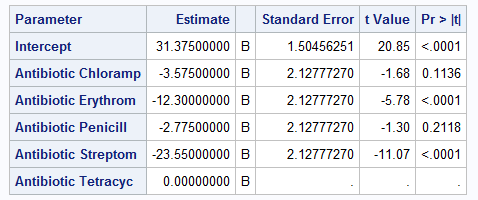
\includegraphics[scale=0.7]{BindFracSolution}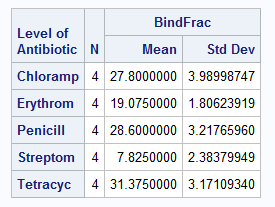
\includegraphics[scale=0.7]{BindFracMeans}
\end{center}

\newpage

Find an estimate of our contrast $\theta=\mu_1-\mu_2$.  Find an estimate for $\theta_6$ and $\theta_8$.\\~\\~\\~\\~\\~\\~\\
We now have a point estimate of the quantity in our null hypothesis, in order to conduct our test we must also know about the variability of this estimate, i.e. What is $\hat{Var}(\hat{\theta})$ or $\hat{SE}(\hat{\theta})$?\\~\\
The variance of a linear combination of means in One-way ANOVA has a very nice form:
 \color{red}{
$$Var(\hat{\theta})=\frac{c_{1}^{2}}{n_{1}}\sigma^2+\frac{c_{2}^{2}}{n_{2}}\sigma^2+...+\frac{c_{t}^{2}}{n_{t}}\sigma^2=\sigma^{2}\sum_{i=1}^{t}\frac{c_{i}^2}{n_{i}}$$
This variance involves the unknown quantity $\sigma^2$.  What value can we use to estimate $\sigma^2$?
$$\hat{Var}(\hat{\theta})=MS(E)\sum_{i=1}^{t}\frac{c_{i}^2}{n_{i}}$$
We can then estimate the standard error by
$$\hat{SE}(\hat{\theta})=\sqrt{MS(E)\sum_{i=1}^{t}\frac{c_{i}^2}{n_{i}}}$$}
\color{black}
Due to the normality assumption on our errors we can use a t-test.  Let $\theta_0$ be a value of interest for our contrast (often 0).  To test $H_{0}:\theta=\theta_{0}$ vs $H_{A}:\theta\neq \theta_{0}$ we can use
        $$t=\frac{\hat{\theta}-\theta_{0}}{\hat{SE}(\hat{\theta})}\sim t_{t(n-1)}~\text{under}~H_{0}$$

What is the value of this test statistic for our contrast $\theta=\mu_1-\mu_2$?  Compare it to $t(0.975,15)=2.13$, what is your conclusion?  What is your interpretation?

\newpage

Likewise a confidence interval can be formed using
$$\hat{\theta}\pm t(\alpha/2,t(n-1))\hat{SE}(\hat{\theta}) = \sum_{i=1}^{t}c_{i}\bar{y}_{i+}\pm t(\alpha/2,t(n-1))\sqrt{MS(E)\sum_{i=1}^{t}\frac{c_{i}^2}{n_{i}}}$$
What is a 95\% CI for $\theta=\mu_1-\mu_2$?  Does your conclusion here match the conclusion using the test statistic?\\~\\~\\~\\~\\~\\~\\~\\~\\

Note:  A contrast that has only two nonzero $c$'s is called a pairwise contrast (as it looks at only two means).  These can be had easily in proc glm using the code below.
\\~\\

A \textbf{complex} contrast is a contrast that involves more than two non-zero coefficients.  For example, $\theta_{10}=\frac{\mu_{1}+\mu_{2}}{2}-\frac{\mu_{3}+\mu_{4}}{2}$ is a complex contrast.  \\~\\

\begin{small}
\begin{verbatim}
proc glm data=binding;
class antibiotic;
model bindfrac=antibiotic/solution;
means antibiotic/ lsd cldiff lines;
lsmeans antibiotic/stderr pdiff;
run;
\end{verbatim}
\end{small}
*Generally we'll want to use lsmeans not means, but ok here since no covariates involved and a balanced design was done.
\begin{center}
\includegraphics[scale=0.65,page=4,trim=60mm 0mm 30mm 0mm ]{BindFracContrasts}\includegraphics[scale=0.65,page=5,trim=30mm 0mm 60mm 0mm ]{BindFracContrasts}\\
\includegraphics[scale=0.65,page=6,trim=60mm 80mm 30mm 0mm ]{BindFracContrasts}\includegraphics[scale=0.65,page=8,trim=30mm 80mm 60mm 0mm ]{BindFracContrasts}\\
\end{center}

Use the output to construct a 95\% CI for $\theta_{10}$.

\newpage

To get the estimate for $\theta_{10}$ (and a few other linear combinations of means) in SAS we can use glm but it will be easiest to use proc mixed:
\begin{small}
\begin{verbatim}
proc glm data=binding;
class antibiotic;
model bindfrac=antibiotic/clparm;
estimate 'lsmean for trt 2' intercept 1 antibiotic 0 1 0 0 0;
estimate 'avg of trt 2 mean and trt 3 mean' intercept 2 antibiotic 0 1 1 0 0/divisor=2;
estimate 'trt 1 vs trt 5' intercept 0 antibiotic 1 0 0 0 -1;
estimate 'avg of 1 and 2 vs avg of 3 and 4' intercept 0 antibiotic 1 1 -1 -1 0/divisor=2;
run;

proc mixed data=binding;
class antibiotic;
model bindfrac=antibiotic;
lsmestimate antibiotic 'lsmean for trt 2' [1,2]/cl;
lsmestimate antibiotic 'avg of trt 2 mean and trt 3 mean' [0.5,2] [0.5,3]/cl;
lsmestimate antibiotic 'trt 1 vs trt 5' [1,1] [-1,5]/cl;
lsmestimate antibiotic 'avg of 1 and 2 vs avg of 3 and 4' [1,1] [1,2] [-1,3] [-1,4]/divisor=2 cl;
run;
\end{verbatim}
\end{small}
\begin{center}
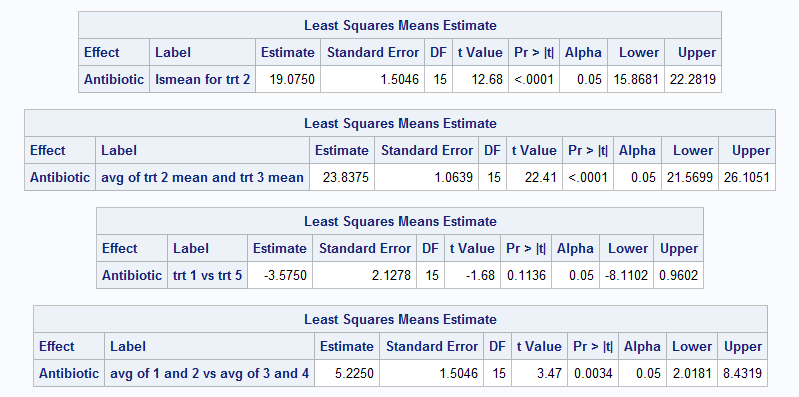
\includegraphics[scale=0.8]{BindFracMixedEstimate}\\
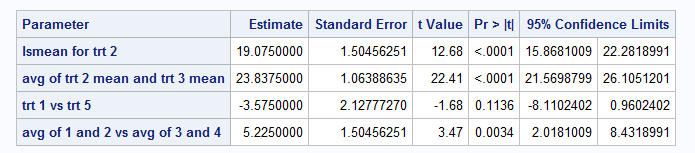
\includegraphics[scale=0.8]{BindFracGLMEstimate}
\end{center}

\newpage

\textbf{Multiple Comparisons Corrections}\\~\\
It is not safe to go carrying out many many significance tests suggested by the data all willy-nilly.  If we do, our \textit{experiment wide} type I error rate will not be controlled.\\~\\
Recall: $\alpha=P(\mbox{Type I Error})$\\
\begin{center}
\begin{tabular}{c|cc}
Decision & $H_0$ true & $H_0$ false\\\hline
Reject $H_0$ & Type I Error & Correct! \\
Fail to Reject $H_0$ & Correct! & Type II Error
\end{tabular}
\end{center}

For a given test, we fix the probability of a type I error to be small (often 0.05) as it is usually considered worse than a type II error.\\~\\
\color{red}{This is similar to the US justice system where we assume innocence until proven guilty.  For most crimes it is much worse to send an innocent person to jail than to let a guilty person go free}\\~\\
\color{black}
Consider the case with $t=5$ (antibiotic treatments): 
\begin{itemize}
\item the number of pairwise contrasts of the form $\theta=\mu_i-\mu_j$ is $\choose{5}{2}=10$
\item each test has type I error $\alpha=0.05$, but overall what is our type I error rate?
$$\mbox{i.e. P(rejecting at least one null hypothesis that is true)}$$
\item This is called the \textit{experimentwise} or \textit{familywise} (fwe) type I error rate.  We should really control this instead of the type I error for each test!\\~\\
\end{itemize}

Example:  Is a certain type of coin fair (equal probability of flipping a head and a tail)?
$$H_0: \mbox{Coin fair}, p=0.5~~~~~~~~~~H_A:\mbox{Coin biased}, p\neq 0.5$$
Experiment - flip one of these coins 10 times, if 9 or 10  heads appear or if 9 or 10 tails appear then declare coin biased.\\~\\
Assuming the coin is fair, 
\begin{eqnarray*}
\alpha & = & P(\mbox{Concluding coin is biased})\\
 & = & P(9~heads)+P(9~tails)+P(10~heads)+P(10~tails)\\
& = & 2*10(1/2)^{10}+2*(1/2)^{10}=0.021
\end{eqnarray*}
This is our type I error rate for testing this particular coin (a little smaller than the usual 0.05).\\~\\
Now suppose we have 100 coins of this type and we test each in the same manner.  If the coins were truly fair, how many of the experiments would we expect to conclude we have a biased coin?\\~\\
For a particular coin to come up heads or tails 9-10 times is very unlikely, but seeing any 1 coin of the 100 behave this way would be more likely than not.\\
In fact, 
$$P(\mbox{All 100 coins identified as fair})=0.34$$
$$P(\mbox{At least 1 coin of the 100 is classsified as biased})=0.66$$
This is why we need to control the fwe rate when we do many data-driven comparisons!\\~\\
\color{red}{In general,
$$\mbox{fwe rate}=P(\mbox{At least 1 type I error})=\alpha^{*}=1-(1-\alpha)^{k}$$
where $k$ is the number of tests being done and $\alpha$ is the significance level used for each test.}\\~\\~\\
\color{black}
Comparisons can be categorized as {\em a priori} or {\em post-hoc}:
\begin{itemize}
\item {\em A priori}: Significance tests which will be carried out without regard to the observed outcome of the experiment.
\item {\em Post-hoc} or data-driven: Significance tests which are suggested by the observed outcome of the experiment.
\end{itemize}

Methods for simultaneous inference for multiple comparisons include (but there are many many of these)
\begin{itemize}
\item Bonferroni
\item \chef
\item Tukey
\end{itemize}

~\\~\\
\textbf{Bonferroni Correction}\\~\\
Suppose interest lies in exactly $k$ contrasts.  \textbf{Bonferroni correction} is to replace the usual $\alpha$ with
$$ \alpha'=\frac{\alpha}{k} $$
By doing so our fwe rate will be less than $\alpha$
$$\mbox{fwe rate}=\alpha^{*}=1-(1-\alpha')^{k}=1-(1-\frac{\alpha}{k})^{k}\leq \alpha$$
We can now create \textbf{simultaneous} CIs.  These are a group of CIs we are $(1-\alpha)$\% confident will \underbar{all} contain their true value.\\~\\
Simultaneous $95\%$ confidence intervals for the $k$ contrasts given by
$$ a_1 \bar{y}_{1+} + a_2 \bar{y}_{2+} + \cdots + a_t \bar{y}_{t+} \pm t(\alpha'/2,t(n-1))\sqrt{MS(E) \sum_{i=1}^{t} \frac{a_i^2}{n_i}} $$
$$ b_1 \bar{y}_{1+} + b_2 \bar{y}_{2+} + \cdots + b_t \bar{y}_{t+} \pm t(\alpha'/2,t(n-1))\sqrt{MS(E) \sum_{i=1}^{t} \frac{a_i^2}{n_i}} $$
$$\vdots$$ 
$$ k_1 \bar{y}_{1+} + k_2 \bar{y}_{2+} + \cdots + k_t \bar{y}_{t+} \pm t(\alpha'/2,t(n-1))\sqrt{MS(E) \sum_{i=1}^{t} \frac{a_i^2}{n_i}} $$
Note: $t(\alpha'/2,t(n-1))$ might have to be obtained using software.\\~\\

For the binding fraction example, consider only pairwise comparisons with Chloramphenicol ($\mu_1$):
$$\theta_1 = \mu_1-\mu_2, ~~~~\theta_2 = \mu_1-\mu_3, ~~~~\theta_3 = \mu_1-\mu_4, ~~~~\theta_4 = \mu_1-\mu_5$$
We have $k=4$, $ \alpha'=0.05/k=0.0125,$ and $t(\alpha'/2,15) = 2.84$.\\~\\
What is the Margin of Error for one of these contrasts?  Find the simultaneous 95\% intervals for the four contrasts.  Which of these antibiotic means differ significantly from the chloramphenicol mean?\\
\color{red}{The Margin of Errors for the CIs are all the same and are, for example,  
$$t_{(\alpha'/2,15)}\sqrt{MS(E) \left(\frac{(1)^2}{4} + \frac{(-1)^2}{4}+\frac{0^2}{4} + \frac{0^2}{4} +\frac{0^2}{4}\right)} = 2.84\sqrt{(9.05)\frac{2}{4}} = 6.043 $$
so that \textit{simultaneous} $95\%$ confidence intervals for $\theta_1,\theta_2,\theta_3,\theta_4$ are
$$\mbox{for }\theta_1:~~~\bar{y}_1-\bar{y}_2 \pm 6.043 = 27.800-19.075 \pm 6.043 = (2.682, 14.768)$$
$$\mbox{for }\theta_2:~~~\bar{y}_1-\bar{y}_3 \pm 6.043 = 27.800-28.600 \pm 6.043 = (-6.836, 5.236)$$
$$\mbox{for }\theta_3:~~~\bar{y}_1-\bar{y}_4 \pm 6.043 = 27.800-~7.825 \pm 6.043 = (13.939, 26.011)$$
$$\mbox{for }\theta_4:~~~\bar{y}_1-\bar{y}_5 \pm 6.043 = 27.800-31.375 \pm 6.043 = (-9.611, 2.461)$$
}
\color{black}
\newpage

\textbf{\chef Correction}\\~\\
\chef correction scales the $t$ multiplier in an interesting way.
$$\mbox{Rather than }t(\alpha/2,t(n-1)) \mbox{ we use }\sqrt{(t-1)F(\alpha,t-1,t(n-1))}$$
**Doesn't depend on the number of contrasts done!\\~\\
For {\bf simultaneous} $95\%$ confidence intervals for {\bf any number} of contrasts, use
$$ \sum_{i=1}^{t} c_i \bar{y}_{i+} \pm \sqrt{(t-1) F(\alpha,t-1,t(n-1)) MS[E] \sum_{i=1}^{t} \frac{c_i^2}{n_i}}$$
For a pairwise comparisons of means, say $\mu_1-\mu_2$, this yields
\begin{large}
$$ \tmean{1} - \tmean{2}\pm \sqrt{(t-1) F(\alpha,t-1,t(n-1)) MS[E] (1/n_1 + 1/n_2)}$$
\end{large}
For binding fraction data, what is the Margin of Error for testing one of the contrasts? (Note: $F(\alpha,t-1,t(n-1))=3.06$)\\
\color{red}{
$$ \sqrt{(t-1) F(\alpha,t-1,t(n-1)) MS[E] \left(\frac{1}{n_i} + \frac{1}{n_j}\right)} = \sqrt{(5-1)(3.06)9.05\left(\frac{1}{4}+\frac{1}{4}\right)} = 7.44$$
(Note: If any two sample means differ by more than 7.44, they differ significantly.)}\\~\\~\\
\color{black}
\textbf{Tukey-Kramer Correction (or just Tukey)}\\~\\
Tukey's correction is the best method when making inference on \textbf{all pairwise} comparisons in balanced designs. That is, for simple contrasts of the form
$$ \theta=\mu_j-\mu_k$$
it will tend to have a lower type II error rate in these cases than \chef and bonferroni corrections.  (It has a greater chance of detecting differences i.e. is more powerful.)
\begin{itemize}
\item Uses multipliers from a distribution called the `studentized range distribution'
\item Denoted $q(\alpha,t,t(n-1))$
\end{itemize}
For {\bf simultaneous} $95\%$ confidence intervals for $\theta=\mu_j-\mu_k$ use
\begin{eqnarray*}
\hat{\theta}&\pm& \frac{q(\alpha,t,t(n-1))}{\sqrt{2}} \hat{SE}(\hat{\theta})\\
\bar{y}_{j+}-\bar{y}_{k+}&\pm& \frac{q(\alpha,t,t(n-1))}{\sqrt{2}}\sqrt{MS(E)(\frac{1}{n}+\frac{1}{n})}\\
\bar{y}_{j+}-\bar{y}_{k+}&\pm& q(\alpha,t,t(n-1))\sqrt{\frac{MS(E)}{n}}
\end{eqnarray*}
\newpage

How to do these multiple comparison corrections in SAS?\\
\begin{itemize}
\item Bonferonni can be done by manually changing the $\alpha$ level SAS uses.  For the example above, $\alpha'=0.05/4=0.0125$:\\
\begin{small}
\begin{verbatim}
proc glm data=binding;
class antibiotic;
model bindfrac=antibiotic/clparm alpha=0.0125;
*Can drop intercept since it has 0 coefficient;
estimate 'theta 1' antibiotic 1 -1; 
estimate 'theta 2' antibiotic 1 0 -1;
estimate 'theta 3' antibiotic 1 0 0 -1 0;
estimate 'theta 4' antibiotic 1 0 0 0 -1;
run;

proc mixed data=binding;
class antibiotic;
model bindfrac=antibiotic;
lsmestimate antibiotic 'theta 1' [1,1] [-1,2]/cl alpha=0.0125;
lsmestimate antibiotic 'theta 2' [1,1] [-1,3]/cl alpha=0.0125;
lsmestimate antibiotic 'theta 3' [1,1] [-1,4]/cl alpha=0.0125;
lsmestimate antibiotic 'theta 4' [1,1] [-1,5]/cl alpha=0.0125;
run;
\end{verbatim}
\end{small}

\item Scheffe and Tukey corrections are options:
\begin{small}
\begin{verbatim}
proc glm data=binding;
class antibiotic;
model bindfrac=antibiotic;
lsmeans antibiotic/pdiff adjust=scheffe cl;
lsmeans antibiotic/pdiff adjust=tukey cl;
run;

proc mixed data=binding;
class antibiotic;
model bindfrac=antibiotic;
lsmeans antibiotic/pdiff adjust=tukey cl;
lsmestimate antibiotic 'theta 1' [1,1] [-1,2]/cl adjust=scheffe;
lsmestimate antibiotic 'theta 2' [1,1] [-1,3]/cl adjust=scheffe;
lsmestimate antibiotic 'theta 3' [1,1] [-1,4]/cl adjust=scheffe;
lsmestimate antibiotic 'theta 4' [1,1] [-1,5]/cl adjust=scheffe;
run;
\end{verbatim}
\end{small}
\end{itemize}

\newpage

Bonferroni GLM output:
\begin{center}
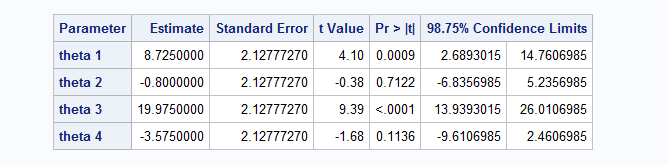
\includegraphics[scale=0.8]{BindFracBon}
\end{center}
Bonferroni Mixed output:
\begin{center}
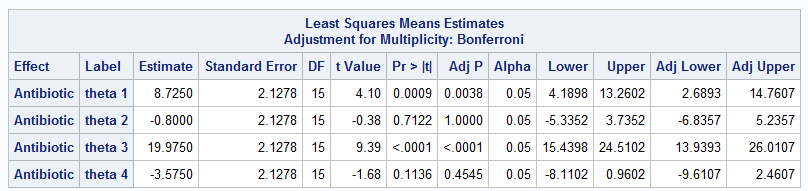
\includegraphics[scale=0.8]{BindFracBonMixed}
\end{center}

\newpage

Scheffe and Tukey GLM output:
\begin{center}
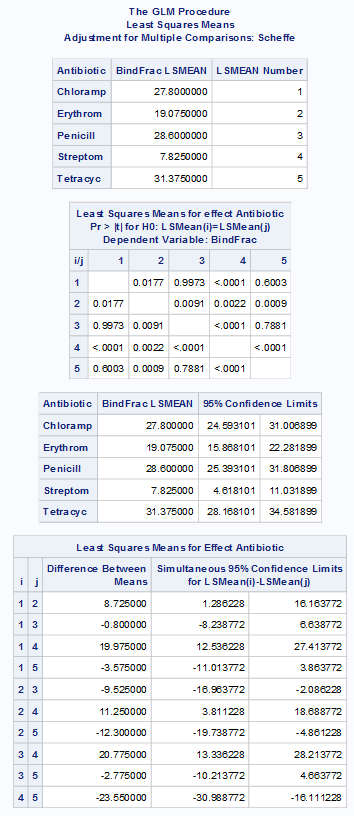
\includegraphics[scale=0.8]{BindFracScheffe}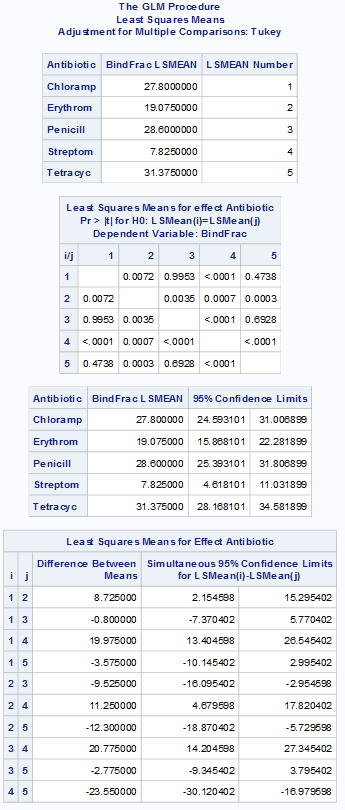
\includegraphics[scale=0.8]{BindFracTukey}
\end{center}

\newpage

Scheffe and Tukey Mixed output:
\begin{center}
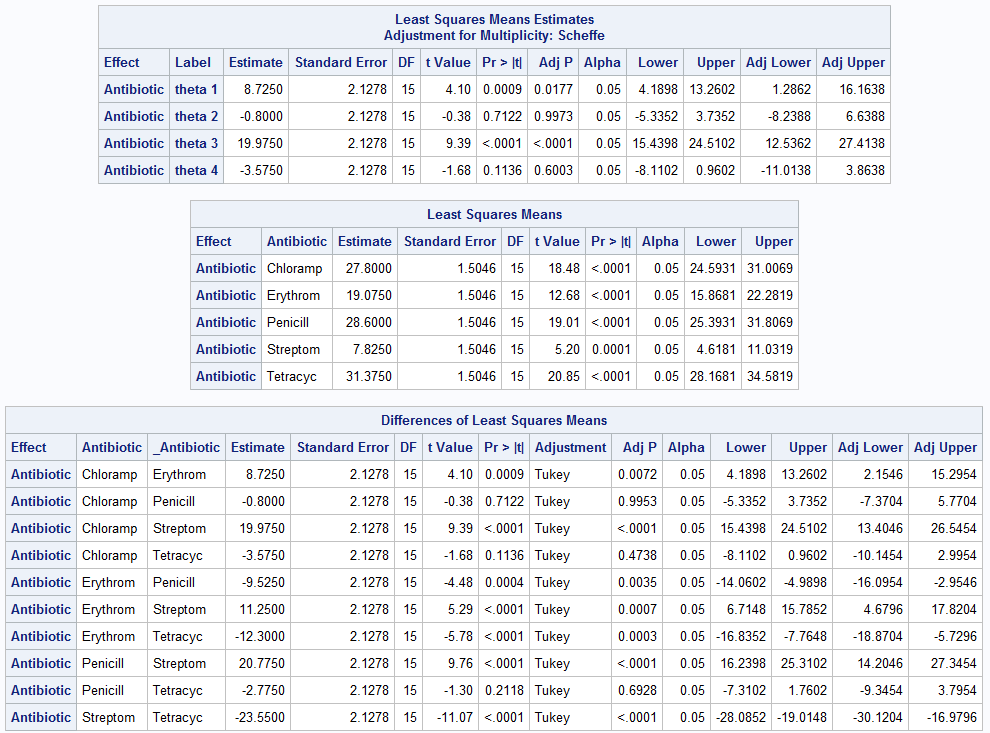
\includegraphics[scale=0.8]{BindFracScheffeTukeyMixed}
\end{center}

\newpage

\textbf{Independent Contrasts}\\

Consider a contrast $\theta$, then
$$\theta=c_{1}\mu_{1}+c_{2}\mu_{2}+...+c_{t}\mu_{t}$$
where $\sum_{i=1}^{t}c_i=0$.  The estimate of a contrast is
$$\hat{\theta}=c_{1}\bar{y}_{1+}+c_{2}\bar{y}_{2+}+...+c_{t}\bar{y}_{t+}$$
and the estimated variance is given by
$$\hat{Var}(\hat{\theta})=MS(E)\sum_{i=1}^{t}\frac{c_i^2}{n_i}$$
Recall: The idea behind ANOVA is that we partition $SS(TOT)$ into independent components $SS(Trt)$ and $SS[E]$.\\~\\
Similarly, we can take $SS(Trt)$ and partition it into $t-1$ independent contrasts each with 1 df.\\~\\

\textbf{Orthogonal contrasts}:\\
Let 
$$\theta_1=\sum_{i=1}^{t}c_i\mu_i \mbox{    and    }\theta_2=\sum_{i=1}^{t}d_i\mu_i$$
be two contrasts.  $\theta_1$ and $\theta_2$ are \textbf{orthogonal} if 
$$c_1d_1+c_2d_2+...+c_td_t=\sum_{i=1}^{t}c_id_i=0$$
A set of $k$ contrasts is mutually orthogonal if all pairs are orthogonal. \\~\\
Examples:\\
$ (-1,1,0,0,0) \mbox{ and } (0,0,-1,1,0) \mbox{ orthogonal ?}$\\~\\
$ (1,-1/2,-1/2,0,0) \mbox{ and } (0,0,0,-1,1) \mbox{ orthogonal ?}$\\~\\
$ (-1,1,0,0,0) \mbox{ and } (0,-1,1,0,0) \mbox{ orthogonal ?}$\\~\\
Due to the joint normality, \textbf{orthogonality implies independence}!  \\~\\

\newpage

\textbf{Sums of squares for contrasts}\\
Recall we are going to partition $SS(Trt)$ into $t-1$ independent contrasts.  The sums of squares for a contrast are
$$ SS(\hat\theta)=\frac{\hat\theta^2}{\left(\frac{c_1^2}{n_1}+\cdots+\frac{c_t^2}{n_t}\right)}=\frac{\hat\theta^2}{\left(\sum_{i=1}^{t}\frac{c_i^2}{n_i}\right)}$$
This contrast has 1 df associated with it.\\~\\
We can define $MS(\hat{\theta})=SS(\hat{\theta})/1=SS(\hat{\theta})$ and can then test
$$H_0:\theta=0~~~~vs~~~~H_A:\theta\neq 0$$
using the F-statistic
$$F=\frac{MS(\hat{\theta})}{MS(E)}\sim F_{1,t(n-1)}$$
Compare this to the $t$-test done earlier for testing a contrast
$$t=\frac{\hat{\theta}-\theta_{0}}{\hat{SE}(\hat{\theta})}\sim t_{t(n-1)}$$
(Remember if we square a $t$ stat we get an $F$ stat!)\\~\\~\\~\\
We can also test multiple contrasts all equal to 0 at once
$$H_0:\theta_1=\theta_2=...=\theta_k=0~~~~vs~~~~H_A:\mbox{At least 1 }\theta\neq 0$$
using the F-statistic
$$F=\frac{\frac{SS(\hat{\theta_1})+SS(\hat{\theta_2})+...+SS(\hat{\theta_k})}{k}}{MS(E)}\sim F_{k,t(n-1)}$$
~\\~\\
How to relate this to $SS(Trt)$? Generally, if $\theta_1,\theta_2,...,\theta_{t-1}$ are $t-1$ mutually orthogonal contrasts then
$$ SS(Trt)=SS(\hat\theta_1)+SS(\hat\theta_2)+\cdots+SS(\hat\theta_{t-1})$$
and $df_{Trt}=df_{\hat\theta_1}+...+df_{\hat\theta_{t-1}}=1+...+1=t-1$\\~\\
Notice, testing all $t-1$ contrasts equal to 0 is equivalent to testing our global $F$-test!\\~\\~\\~\\

Again consider the Binding Fraction data.  In this case we have $5-1=4$ df for treatment.  Consider the following set of 4 mutually orthogonal contrasts:
\begin{eqnarray*}
\theta_1&=&(-2~~-1~~~~0~~~~~1~~~~2)\\
\theta_2&=&(2~~~~-1~-2~~-1~~~~2)\\
\theta_3&=&(-1~~~~~2~~~~0~~-2~~~~1)\\
\theta_4&=&(1~~~~-4~~~~6~~-4~~~~1)
\end{eqnarray*}
Since these are mutually orthogonal, they are all independent.\\

Let's use SAS to get estimates.  Test for $\theta_4=0$ using both the $t$ and $F$ tests.  Then show that $SS(Trt)=SS(\theta_1)+SS(\theta_2)+SS(\theta_3)+SS(\theta_4)$ and conduct the global $F$ test.\\~\\~\\~\\~\\~\\~\\~\\
\begin{small}
\begin{verbatim}
proc glm data=binding; class antibiotic; model bindfrac=antibiotic;
contrast 'theta 1' antibiotic -2 -1 0 1 2;
contrast 'theta 2' antibiotic 2 -1 -2 -1 2;
contrast 'theta 3' antibiotic -1 2 0 -2 1;
contrast 'theta 4' antibiotic 1 -4 6 -4 1; run;

proc mixed data=binding; class antibiotic; model bindfrac=antibiotic;
lsmestimate antibiotic 'theta 1' [-2,1] [-1,2] [0,3] [1,4] [2,5]; 
lsmestimate antibiotic 'theta 2' [2,1] [-1,2] [-2,3] [-1,4] [2,5]; 
lsmestimate antibiotic 'theta 3' [-1,1] [2,2] [0,3] [-2,4] [1,5]; 
lsmestimate antibiotic 'theta 4' [1,1] [-4,2] [6,3] [-4,4] [1,5]; run;
\end{verbatim}
\end{small}

\begin{center}
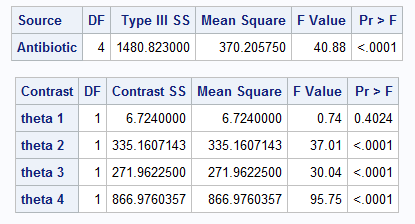
\includegraphics[scale=0.75]{BindFracContrastSS}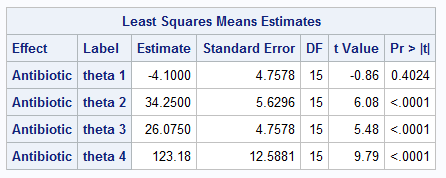
\includegraphics[scale=0.7]{BindFracContrastMixed}
\end{center}

\newpage
Consider a new dataset:  Data consists of the number of contaminants in IV fluids made by $t=3$ pharmaceutical companies
\begin{center}
\begin{tabular}{c|ccc|} \hline
&Cutter & Abbott & McGaw \\ \hline
&255 & 105 & 577 \\
&264 & 288 & 515 \\
&342 & 98 & 214 \\
&331 & 275 & 413 \\
&234 & 221 & 401 \\
&217 & 240 & 260 \\ \hline
$\tmean{i}$ &273.8 & 204.5 & 396.7 \\ \hline
\end{tabular}
\end{center}
\bigkn
\begin{center}
\begin{tabular}{|c|c|c|c|c|}  \hline
& & Sum of & Mean & \\
Source & d.f. & squares & Square & F \\ \hline
Treatments (or pharmacies) & $2$ & 113646 & 56823 & 5.81\\
Error & $15$ & 146753 & 9784 & \\
Total & 17 & 260400 & & \\ \hline
\end{tabular}
\end{center}
Consider the following 2 contrasts:
$$ \theta_1 = \mu_M-\mu_A \ \ \ \mbox{ and }\ \ \ \theta_2=\mu_C-\frac{\mu_M+\mu_A}{2}$$
Which levels of the factor will each of these be in SAS? Rewrite these contrasts in terms of $\mu_1$, $\mu_2$, and $\mu_3$.\\~\\~\\~\\~\\
Are these contrasts orthogonal?\\~\\~\\~\\
Are the estimated contrasts $\hat\theta_1$ and $\hat\theta_2$ independent?\\~\\~\\
Use the output to compute $SS(\hat\theta_1)$ and $SS(\hat\theta_2)$.  What should these add up to and why?

\newpage

\begin{small}
\begin{verbatim}
proc glm data=pharm; class company; model contam=company;
contrast 'McGaw vs Abbot' company -1 0 1;
estimate 'McGaw vs Abbot'  company -1 0 1;
contrast 'Cutter vs avg of McGaw and Abbot' company -1 2 -1;
estimate 'Cutter vs avg of McGaw and Abbot' company -1 2 -1/divisor=2; run;
\end{verbatim}
\end{small}
 Note: We should really do a multiple comparison correction for our two contrasts.  Bonferonni is easiest, compare our p-values to $0.05/2=0.025$.
\begin{center}
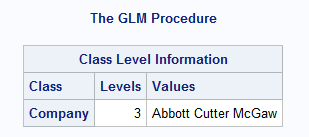
\includegraphics[scale=0.8]{PharmGLM1}\\
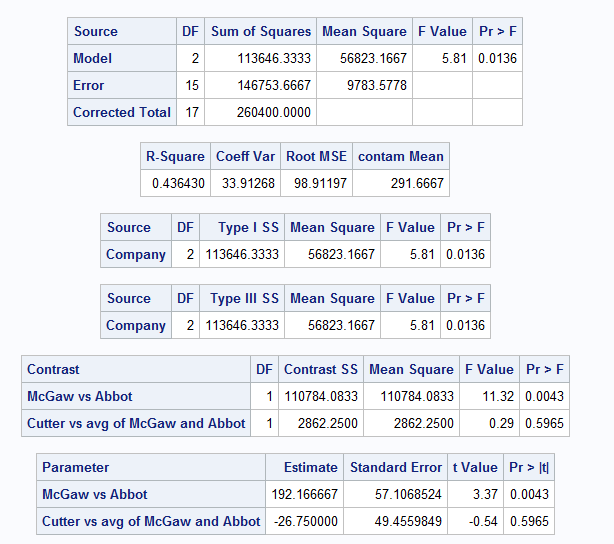
\includegraphics[scale=0.8]{PharmGLM2}\\

\includegraphics[scale=0.8]{PharmGLM3}
\end{center}

\newpage

\textbf{Polynomial contrasts} \\
For one-way ANOVA, if the factor is actually on the interval scale but observed at only a few levels we can test for polynomial relationships.\\~\\
With $t$ levels, we can fit any polynomial of degree $t-1$ or less.  (Polynomial of degree $t-1$ is equivalent to fitting ANOVA model.)  That is, every polynomial model of degree $t-2$ or less is nested in the full ANOVA model!\\~\\
Example: A poultry science experiment measures bodyweights of chickens from $t=4$ diet groups.  Diets are characterized by protein concentration in diet.
\begin{itemize}
\item Response $Y$ = 21-day bodyweights of chickens 
\item A balanced CRD was done with diet and $N=72$ total chickens.  (Implying $n=18$).
\end{itemize}
Experiment Summary:
\begin{center}
\begin{tabular}{ccc}
diet group & $x$: level of protein & diet mean $\bar{y}_{i+} $\\\hline                                                                                
1 &              21.8         & 994.9       \\
2 &              23.5         & 1000.6 \\
3 &              25.2         & 1025.8 \\
4 &              26.9         & 1056.0\\ 
\hline
\end{tabular}
\end{center}
Here we can see that our factor is actually on an interval scale but measured at only 4 levels.  \\~\\
Consider the One-way ANOVA model using diet and the Linear Regression model cubic in protein:
\begin{small}
\begin{verbatim}
proc glm data=chickens; class diet;
model gain=diet; run;

proc glm data=chickens;
model gain=protein protein*protein protein*protein*protein; run;
\end{verbatim}
\end{small}

\begin{center}
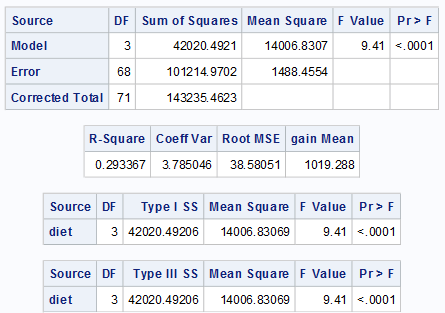
\includegraphics[scale=0.8]{ChickensGLM}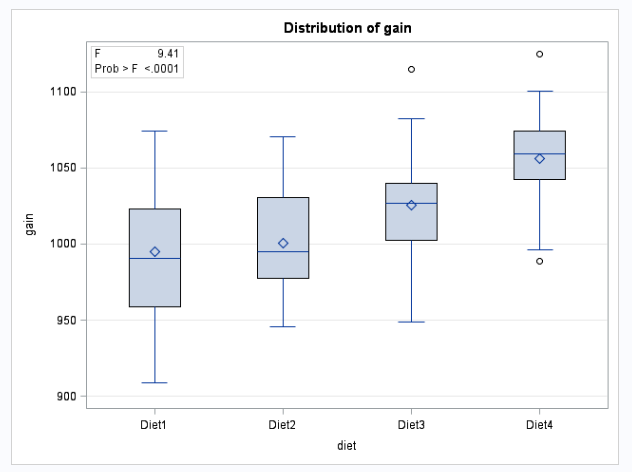
\includegraphics[scale=0.5]{ChickensBoxPlot}\\
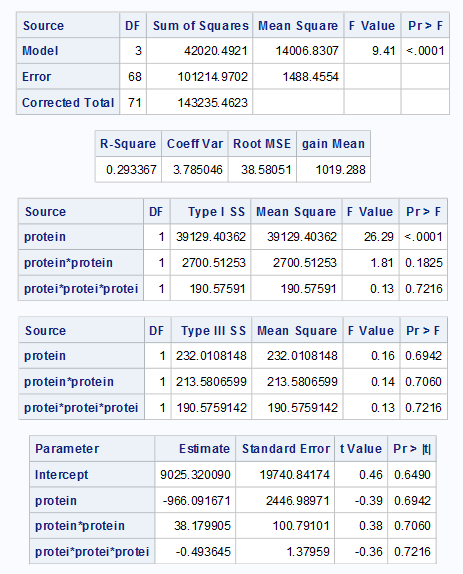
\includegraphics[scale=0.8]{ChickensGLM2}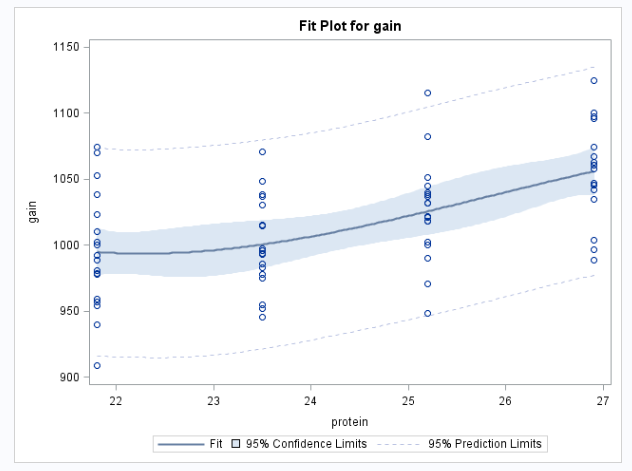
\includegraphics[scale=0.5]{ChickensScatter}
\end{center}

Investigate the two ANOVA tables.  Also inspect the Type I Sums of Squares for the MLR model, these would be useful in model building!  We can test for the adequacy of a model linear or quadratic in protein rather than the full ANOVA (equivalent to the cubic model).\\~\\

\newpage 
If we have equally spaced levels (differences between levels all the same), we can actually write down the different polynomial parts in terms of contrasts.  Below gives the contrasts you would use for equally spaced levels for 3, 4, or 5 levels.
\begin{center}
\begin{tabular}{ccc|ccccc|c}
Factor& Poly.& & \multicolumn{5}{c|}{Coefficients for} & \\
levels & Degree & contrast & $\bar{y}_{1+}$ & $\bar{y}_{2+}$ & $\bar{y}_{3+}$ & $\bar{y}_{4+}$ & $\bar{y}_{5+}$ & $SS(\hat\theta_i)$\\ \hline
3 & 1 &$\hat\theta_1$& -1 & 0 & 1 & & & $R(\beta_1|\beta_0)$\\
  & 2 &$\hat\theta_2$& 1 & -2 & 1 & & & $R(\beta_2|\beta_0,\beta_1)$\\ \hline
4 & 1 &$\hat\theta_1$& -3 & -1 & 1 & 3 & & $R(\beta_1|\beta_0)$\\
  & 2 &$\hat\theta_2$& 1 & -1 & -1 & 1 & & $R(\beta_2|\beta_0,\beta_1)$\\ 
  & 3 &$\hat\theta_3$& -1 & 3 & -3 & 1 & & $R(\beta_3|\beta_0,\beta_1,\beta_2)$\\  \hline
5 & 1 &$\hat\theta_1$& -2 & -1 & 0 & 1 & 2 & $R(\beta_1|\beta_0)$\\
  & 2 &$\hat\theta_2$& 2 & -1 & -2 & -1 & 2 & $R(\beta_2|\beta_0,\beta_1)$\\
  & 3 &$\hat\theta_3$& -1 & 2 & 0 & -2 & 1 & $R(\beta_3|\beta_0,\beta_1,\beta_2)$\\
  & 4 &$\hat\theta_4$& 1 & -4 & 6 & -4 & 1 & $R(\beta_4|\beta_0,\beta_1,\beta_2,\beta_3)$\\ \hline
\end{tabular}
\end{center}

Rightmost column indicates extra SS in MLR of the form
$$\mu(x) = \beta_0 + \beta_1 x + \beta_2 x^2 + \cdots.$$
The contrast corresponding to a polynomial of degree $p$
can be used to test for a $p^{th}$ degree association:

\begin{itemize}
\item large $|\hat\theta_1|$ indicates
linear association between $y$ and $x$.
\item large $|\hat\theta_2|$ indicates
quadratic association between $y$ and $x$.
\item large $|\hat\theta_3|$ indicates 
cubic association between $y$ and $x$.
\end{itemize}

\begin{small}
\begin{verbatim}
proc glm data=chickens; class diet; model gain=diet;
contrast 'linear' diet -3 -1 1 3;
contrast 'quadratic' diet 1 -1 -1 1;
contrast 'cubic' diet -1 3 -3 1; run;
\end{verbatim}
\end{small}

\begin{center}
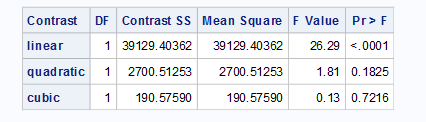
\includegraphics[scale=0.8]{ChickensGLM3}
\end{center}

Note the equivalence between this output and the linear regression model cubic in protein.  Conclusion?  Go ahead and use the linear model rather than the full ANOVA.  No need to look at pairwise comparisons etc.\\~\\

\textbf{$F$-ratio for lack-of-fit:}\\ 
To test for lack-of-fit of a polynomial ({\em reduced}) model of degree $p$, use extra sum-of-squares F-ratio on $t-1-p$ and $N-t$ $df$:
$$ F=\frac{SS(\mbox{lack of fit})/(t-1-p)}{MS(E)_{full}}$$
where
\begin{eqnarray*}
SS(\mbox{lack-of-fit})  &=&  SS(Trt)-SS(R)_{poly} \\
&=&  SS(E)_{poly}-SS(E)_{full}
\end{eqnarray*}

For illustration purposes (i.e. this isn't necessary), let's test if the quadratic model is sufficient or if the full ANOVA model is necessary.
\color{red}{
$$SS(\mbox{lack-of-fit})=42020.49-(39129.40+2700.51)=190.58$$
$$MS(E)_{full}=1488.46$$
This implies
$$F=\frac{SS(\mbox{lack of fit})/(4-1-2)}{MS(E)_{full}}=190.58/1488.46=0.128$$
Fail to reject that the full ANOVA model is necessary.  That is, the quadratic model does not suffer from lack of fit.
}
\color{black}



